\documentclass[12pt]{exam}

\newcommand{\course}{MTH 234 Summer 2021}
\newcommand{\qdate}{Stokes Theorem} %PUT DATE HERE
\newcommand{\quiz}{Group Work} 
\newcommand{\mbf}{\mathbf{F}}

    \usepackage[top=1in, bottom=1in, left=.45in, right=.45in]{geometry}
    \usepackage{amsmath,amsthm,amssymb,amstext}
    \usepackage{enumerate,enumitem}
    \usepackage{tikz,float,graphicx}
    \usepackage{microtype}
    \usepackage{bm,tikz}
        \usetikzlibrary{calc,positioning}
    \usepackage{multicol}
    \usepackage{nicematrix}
    \usepackage{cleveref}
    \usepackage[framemethod=tikz]{mdframed}
    \usepackage{graphicx}
    \usepackage[export]{adjustbox}
    
    %\newcommand{\course}{MTH 234 Summer 2021}
    %\newcommand{\qdate}{Equations of lines and planes} %PUT DATE HERE
    %\newcommand{\quiz}{Group Work} 
    
    \newcommand{\R}{\mathbb{R}}
    
    \newcommand{\ba}{\bm{a}}
    \newcommand{\bb}{\bm{b}}
    \newcommand{\bc}{\bm{c}}
    \newcommand{\bi}{\bm{i}}
    \newcommand{\bj}{\bm{j}}
    \newcommand{\bk}{\bm{k}}
    \newcommand{\br}{\bm{r}}
    \newcommand{\bv}{\bm{v}}
    \newcommand{\bu}{\bm{u}}
    \newcommand{\gen}[1]{\left\langle #1 \right\rangle}
    \newcommand{\pd}[2]{\dfrac{\partial #1}{\partial #2}}

\newtheorem*{theorem}{Theorem}
\surroundwithmdframed[]{theorem}

\theoremstyle{definition}
    \newtheorem*{definition}{Definition}
    \surroundwithmdframed[]{definition}
    \newtheorem*{info}{Useful Information}
    \surroundwithmdframed[]{info}
\theoremstyle{remark}
    \newtheorem*{remark}{Remark}
    \surroundwithmdframed[]{remark}
    

%%%%%%%%%%%%%%%%%%%%%%%
% HEADER AND FOOTER
%%%%%%%%%%%%%%%%%%%%%%%
\pagestyle{headandfoot}
\firstpageheadrule
\runningheadrule
\firstpageheader{\course}{\quiz}{\qdate}
\runningheader{\course}{\quiz}{\qdate}
\runningfooter{}{}{}


\usepackage{color}
\shadedsolutions
\definecolor{SolutionColor}{rgb}{0.8,0.9,1}

\usepackage{pgfplots}
    \pgfplotsset{every axis/.append style={
                    axis x line=middle,    % put the x axis in the middle
                    axis y line=middle,    % put the y axis in the middle
                    axis z line=middle,
                    axis line style={<->}, % arrows on the axis
                    xlabel={$x$},          % default put x on x-axis
                    ylabel={$y$},          % default put y on y-axis
                    zlabel={$z$},
                    grid=both,
                    %xtick={-4,...,-1,1,...,3},
                    %ytick={-1,1,}
    }}
    \pgfplotsset{compat=1.17}

\newcommand{\bif}{\quad\iff\quad}

%\printanswers
\noprintanswers

\begin{document}

\section*{\qdate}

%\subsection*{Template}

\begin{theorem}[Stokes Theorem]
    Let \(S\) be an oriented piecewise-smooth surface that is bounded by a simple, closed, piecewise-smooth boundary curve \(C\) with positive orientation. Let \(\mathbf{F}\) be a vector field whose components have continuous partial derivatives on an open region in \(\R^3\) that contains \(S.\) Then
    \[
        \int_{C}\mathbf{F}\cdot d\bm{r} = \iint_S \mathrm{curl}~\mathbf{F}\cdot d\mathbf{S}
    \]
\end{theorem}

\noindent \textbf{The following is a list of the results you should get for the associated exercise}:
\begin{enumerate}
    \item \(16\pi\) two times.
    \item \(0\)
    \item \(81\pi/2\)
    \item Satisfaction and a better understanding of this section's material.
    \item More of the above
\end{enumerate}

\subsection*{Exercises}
\begin{questions}

\question 
    Evaluate \(\iint_S~\mathrm{curl}~\mbf~d\mathbf{S}\) where
    \(\mbf(x,y,z)=-y\bi+x\bj-2\bk\) and \(S\) is the cone \(z^2=x^2+y^2\) with \(0\le z\le 4\).

    Then, verify Stokes' theorem is true for \(\mbf\) and \(S\) by evaluating \(\int_C~\mbf\cdot d\bm{r}\).
    \ifprintanswers

        \begin{solution}
        We first compute \(\iint_S~\mathrm{curl}~\mathbf{F}\cdot d \mathbf{S}\).
        \begin{align*}
            \mathrm{curl}~\mbf & = \nabla\times\gen{-y,x,-2}\\
                & = \gen{0,0,2}
        \end{align*}
        Viewing \(S\) as a graph with \(z=g(x,y)=\sqrt{x^2+y^2}\) over \(D=\{(x,y)|x^2+y^2\le 4\}\),
        \begin{align*}
            \iint_S~\mathrm{curl}~\mbf~d\mathbf{S} & = \iint_D \left(-(-y)\pd{z}{x}-(x)\pd{z}{y}+(-2)\right)~dA\\
                & = \int_D xy/\sqrt{x^2+y^2}-xy/\sqrt{x^2+y^2}-2~dA\\
                & = -2\int_D~dA
        \end{align*}
        Since \(D\) is a cirle of radius \(4\), the result is \(-2\pi(4)^2=-32\pi\). However, the above assumed upward orientation, so the actual result is
        \[
            \boxed{\iint_S~\mathrm{curl}~\mathbf{F}\cdot d \mathbf{S} = 32\pi}
        \]


        We now evaluate 
        Let \(C\) be the curve of intersection between the cone and the plane \(z=4\).
        Then \(C\), oriented counterclockwise, is given by 
        \[
            \bm{r}(t) = \gen{4\cos t,4\sin t,4},~~0\le t\le 2\pi.
        \]
        \begin{align*}
            \iint_S~\mathrm{curl}~\mathbf{F}\cdot d\mathbf{S} & = \int_C~\mbf\cdot d\bm{r}\\
                & = \int_0^{2\pi} \mbf(\bm{r}(t))\cdot \bm{r}'(t)~dt\\
                & = \int_0^{2\pi} \gen{-4\sin t,4\cos t,-2}\cdot \gen{-4\sin t,4\cos t,0}~dt\\
                & = \int_0^{2\pi} 16\sin^2t+16\cos^2t~dt \\
                & = \int_0^{2\pi}16~dt\\
                & = 32\pi.
        \end{align*}

    \end{solution}
    \else
        \vfill
    \fi

\newpage 
\question Evaluate \(\iint_S~\mathrm{curl}~\mbf\cdot d\mathbf{S}\) using Stokes' Theorem where 
        \(\mbf=x^2z^2\bi+y^2z^2\bj+xyz\bk\) and \(S\) is the part of the paraboloid \(z=x^2+y^2\) that lies in the cylinder
        \(x^2+y^2=4\), oriented upward.
    \ifprintanswers
        \begin{solution}
            The boundary of \(S\) is the curve \(C\) defined by \(x^2+y^2=4\) restricted to the plane \(z=4\). \(C\) can be parameterized by 
            \(\bm{r}(t)=\gen{\cos t,\sin t,4}\).
            By Stokes' Theorem
        \begin{align*}
        \iint_S \mathrm{curl}~\mathbf{F}\cdot d\mathbf{S} 
            & = \int_{C}\mathbf{F}\cdot d\bm{r}\\
            & = \int_0^{2\pi}\mbf(\bm{r}(t))\cdot \bm{r}'(t)~dt\\
            & = \int_0^{2\pi}\gen{16\cos^2(t),16\sin^2(t),4\sin(t)\cos(t)}\cdot \gen{-\sin(t),\cos(t),0}~dt\\
            & = \int_0^{2\pi}-16\sin(t)\cos^2(t)+16\cos(t)\sin^2(t)~dt\\
            & = 0
        \end{align*}
        \end{solution}
    \else
        \vfill
    \fi






%%%%%%%%%%%%%%%%%%


\question Use Stokes' Theorem to evaluate 
\(\int_C\mathbf{F}\cdot d\bm{r}\) where \(\mbf(x,y,z)=\gen{x^2z,xy^2,z^2}\) and \(C\) is the 
curve of intersection of the plane \(x+y+z=1\) and the cylinder \(x^2+y^2=9\) oriented counterclockwise when viewed from above.
    \ifprintanswers
        \begin{solution}
            \begin{align*}
                \mathrm{curl}~\mbf & = \nabla\times\gen{x^2z,xy^2,z^2}\\
                    & = \gen{0-0,-0+x^2,y^2-0}\\
                    & = \gen{0,x^2,y^2}
            \end{align*}
            Any surface bounded by \(C\) will work, but we will use the surface \(x+y+z=1\) with the restriction \(x^2+y^2\le 9\) and viewed as a graph \(z=g(x,y)=1-x-y.\)
            Then 
            \begin{align*}
                \iint_{S}~\text{curl}~\mbf~dS & = \iint_D \left( -(0)\pd{g}{x}-x^2\pd{g}{y}+y^2 \right)~dA\\
                    & = \iint_D x^2+y^2~dA\\
                    & = \int_{0}^{2\pi}\int_0^3~r^3~dr~d\theta\\
                    & =  (2\pi)\left(\frac{3^4}{4}\right)\\
                    & = \boxed{\frac{81}{2}\pi}
            \end{align*}
        \end{solution}
    \else
        \vfill
    \fi

\newpage

\question Show that if \(S\) is a sphere and \(\mbf\) is a vector field that satisfies the conditions for Stokes' theorem everywhere, then 
\[
    \iint_S~\mathrm{curl}~\mbf\cdot d\mathbf{S} = 0.
\]
\emph{Hint: The sphere can be thought of as two half-sphere's sharing a common boundary. Think carefully about how the boundary is oriented on each half if the sphere is oriented outward.}
    \ifprintanswers
        \begin{solution}
            We divide the sphere into two half-spheres \(H_1\) and \(H_2\), the upper and lower halves respectively. 
            Let \(C\) be the shared boundary of the two halves. Let \(C_1\) and \(C_2\) denote \(C\) oriented as determined by the orientation of \(H_1\) and \(H_2\) respectively.

            By stokes' theorem 
            \begin{align*}
                \iint_S~\mathrm{curl}~\mbf\cdot d\mathbf{S} 
                    & =  \iint_{H_1}~\mathrm{curl}~\mbf\cdot~d\mathbf{S}+\iint_{H_2}~\mathrm{curl}~\mbf\cdot~d\mathbf{S}\\
                    & = \iint_{C_1}~\mbf\cdot d\bm{r}+\iint_{C_2}~\mbf\cdot d\bm{r}
            \end{align*}
        Since the sphere is oriented outwardly, \(C_2=-C_1\). Therefore
        
        \begin{align*}
            \iint_{C_1}~\mbf\cdot d\bm{r}+\iint_{C_2}~\mbf\cdot d\bm{r} 
                & = \iint_{C_1}~\mbf\cdot d\bm{r}+\iint_{-C_1}~\mbf\cdot d\bm{r}\\
                & = \iint_{C_1}~\mbf\cdot d\bm{r}-\iint_{C_1}~\mbf\cdot d\bm{r}\\
                & = 0.
        \end{align*}
        \end{solution}
    \else
        \vfill
    \fi

\newpage 

\question Let \(C\) be any simple closed smooth curve that lies in the plane \(x+y+z=1\). 
Show that the line integral 
\[
        \int_C z~dx-2x~dy+3y~dz
\]
depends only on the area of the region enclosed by \(C\) and not on the shape of \(C\) or its location in the plane above.
    \ifprintanswers
        \begin{solution}
        \begin{align*}
            \int_C z~dx-2x~dy+3y~dz & = \int_C \gen{z,-2x,3y}\cdot\gen{dx,dy,dz}\\
                & = \int_C \gen{z,-2x,3y}\cdot d\bm{r}.
        \end{align*}
        Let \(S\) be any surface bounded by \(C\). 
        Let \(D\) be the part of the plane \(x+y+z=1\) bounded by \(C\). 

        By stokes theorem,
        \[
            \int_C \mbf \cdot d\bm{r} = \iint_S~\mathrm{curl}~\mbf~d\mathbf{S}.
        \]

        We have 
        \begin{align*}
            \mathrm{curl}~\mbf & = \nabla \times \gen{z,-2x,3y}\\
                & = \gen{3-0,1-0,-2-0}\\
                & = \gen{3,1,-2}.
        \end{align*}
        A normal vector to the plane \(x+y+z=1\) is \(\bm{n}=\gen{1,1,1}\). So
        \begin{align*}
            \iint_S~\mathrm{curl}~\mbf~d\mathbf{S} 
                & = \iint_S~\mathrm{curl}~\mbf \cdot \bm{n}~dS\\
                & = \iint_S\gen{3,1,-2}\cdot\gen{1,1,1}~dS\\
                & = 2~\iint_S~1~dS.
        \end{align*}
        If \(z=g(x,y)=1-x-y\) and \(f(x,y,z)=1\),
        \begin{align*}
            2~\iint_S~1~dS &= 2\iint_S~f(x,y,z)~dS\\
                & = 2\iint_D~f(x,y,g(x,y))~dA\\
                & = 2\iint_D~1~dA\\
                & = 2\cdot\text{Area}(D).
        \end{align*}

        Therefore the initial line integral depends only on the area of the subsurface of \(z=1-x^2-y^2\) bounded by \(C\). Futhermore, if \(C_1\) and \(C_2\) are different curves in the plane \(x+y+z=1\) and they both bound subsurfaces with area \(A\),
            \[
                \int_{C_1} z~dx-2x~dy+3y~dz = 2A = \int_{C_2} z~dx-2x~dy+3y~dz.
            \]
        \end{solution}
    \else
        \vfill
    \fi

\end{questions}

\end{document}

% soln : Question environment
    \ifprintanswers
        \begin{solution}
        \end{solution}
    \else
        \vfill
    \fi



    \part \(\mbf(x,y,z)=\gen{yz,2xz,e^{xy}}\)\\
    \(C\) is the circle \(x^2+y^2=16,z=5\).
    \ifprintanswers
        \begin{solution}
            If \(S\) is the surface defined by \(x^2+y^2\le 16,z=5\) then \(\int_C\mathbf{F}\cdot d\bm{r}=\iint_S~\mathrm{curl}~\mbf\cdot d\bm{S}\).
            We can think of this as the graph of the function \(z=5\) over the \(D\), the solid disk \(x^2+y^2\le 16\).%, which can be expressed by \(\{(r,\theta)|0\le r \le 4,0\le \theta < 2\pi\}\).

            Then 
            \begin{align*}
                \int_C\mathbf{F}\cdot d\bm{r} & = \iint_S\mbf\cdot d\bm{S}\\
                    & = \iint_D \left( -(yz)\pd{g}{x}-(2xz)\pd{g}{y}+e^{xy} \right)~dA\\
                    & = \iint_D e^{xy}~dA
            \end{align*}
            where the last equality follows from \(\pd{g}{x}=\pd{g}{y}=0\).

            Then 

            \[
                \iint_D e^{xy}~dA = \int_0^{2\pi}\int_0^4~r\cdot e^{r^2\cos\theta\sin\theta}~dr~d\theta
            \]
        \end{solution}
    \else
        \vfill
    \fi


\part \(\mbf=xyz\bi+xy\bj+x^2yz\bk\)\\
    \(S\) is the cube with vertices \((\pm1,\pm1,\pm1)\) without the bottom side (i.e. the square with vertices \((\pm1,\pm1,-1)\)).\\
    \emph{Hint: This is easier than it might seem if you remember the appropriate theorem about line integrals.}
    \ifprintanswers
        \begin{solution}
            The boundary of this surface is the square shown below in the plane \(z=-1\), with 
            \(C=L_1\cup L_2\cup L_3\cup L_4\).
            \begin{center}
                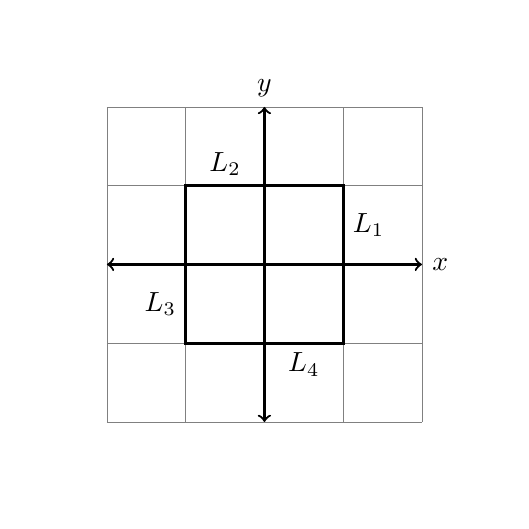
\begin{tikzpicture}
                \draw[white,fill=white] (-3,-3)--(3,-3)--(3,3)--(-3,3)--(-3,-3);
                \draw[gray,very thin] (-2,-2) grid[step=1] (2,2);
                \draw[thick,<->] (-2,0)--(2,0) node[right] {$x$};
                \draw[thick,<->] (0,-2)--(0,2) node[above] {$y$};
                %\draw[very thick] (-1,-1)--(1,-1)--(1,1)--(-1,1)--(-1,-1);
                \draw[very thick] (-1,-1) rectangle (1,1);
                \node[right] at (1,.5) {$L_1$};
                \node[above] at (-.5,1) {$L_2$};
                \node[left] at (-1,-.5) {$L_3$};
                \node[below] at (.5,-1) {$L_4$};
                \end{tikzpicture}
            \end{center}
            Since \(C\) is a simple closed path, Stokes' theorem gives us,
                \[
                    \iint_S~\text{curl}~\mbf\cdot d\mathbf{S} = \int_C\mbf\cdot d\bm{r} = 0.
                    \]

       \end{solution}
    \else
        \vfill
    \fi